\section{Local disk model}
We study the local stability of an inviscid, self-gravitating and
magnetized barotropic fluid disk orbiting a central mass with
potential $\Phi_*(r,z)$, where $(r,\varphi,z)$ are cylindrical
co-ordinates from the central mass. We use the shearing box approximation     
\citep{goldreich65b} and consider a small patch of the disk at
$r=r_0$. The local frame rotates at angular velocity 
$\Omega_0=\Omega(r_0,0)$ about the central mass, where $r\Omega^2 =
\p\Phi_*/\p r$. We also define $S=-r\p\Omega/\p r$ as the local shear
rate and $\Omega_z^2\equiv\p^2\Phi_*/\p z^2$ as the square of the
local vertical frequency. 

A Cartesian co-ordinate system $(x,y,z)$ is set
up in this local frame, corresponding to the radial, azimuthal and vertical
directions of the global disk, respectively. The shearing box fluid
equations read 
\begin{align} 
  &\frac{\p\rho}{\p t}+\nabla\cdot(\rho\bm{v}) = 0,\\
  &\frac{\p \bm{v}}{\p t} + \bm{v}\cdot\nabla\bm{v} +
  2\Omega_0\hat{\bm{z}}\times\bm{v} = - \frac{1}{\rho}\nabla\Pi +
  \frac{1}{\rho\mu_0}\bm{B}\cdot\nabla\bm{B}
  -\nabla\Phi,\\
  &\frac{\p\bm{B}}{\p t}= \nabla\times\left(\bm{v}\times\bm{B} -
  \eta\nabla\times\bm{B}\right), 
\end{align}
where $\rho$ is the density field; $\bm{v}$ is the total velocity in
the local frame; $\bm{B}$ is the magnetic field which satisfies
$\nabla\cdot\bm{B}=0$; $\Pi \equiv P +
|\bm{B}|^2/2\mu_0$ is the total pressure ($\mu_0$ is the vacuum
permeability) and $P=P(\rho)$ is the gas pressure given by a
barotropic equation of state chosen later.  

The total potential is $\Phi = \Phi_\mathrm{ext} + \Phi_d$, where
\begin{align}
  \Phi_\mathrm{ext}(x,z) = -\Omega_0 S_0 x^2 +
  \frac{1}{2}\Omega_{z0}^2z^2 
\end{align}
is the effective external potential (central plus centrifugal) in the
shearing box approximation, where $S_0\equiv S(r_0,0)$ and
$\Omega_{z0}\equiv\Omega_z(r_0,0)$; 
%% \begin{align}
%%   S\equiv -r\frac{\p\Omega}{\p r}, \quad\quad \Omega_{z0}^2\equiv
%%   \frac{\p^2\Phi_*}{\p z^2} 
%% \end{align}
%is the local shear rate and vertical frequency respectively; 
and the gas potential $\Phi_d$ statisfies Poisson's equation
\begin{align}
  \nabla^2\Phi_d = 4\pi G \rho, 
\end{align}
where $G$ is the gravitational constant. For clarity, hereafter we
drop the subscript $0$ on the frequencies. 

\subsection{Self-gravitating equilibria} 
The unperturbed disk is steady and described by
$\rho=\rho(z)$, $\bm{B} = B\hat{\bm{z}}$ where $B$ is a constant, and
velocity field $\bm{v} = -Sx\hat{\bm{y}}$. We have assumed a thin disk 
and neglected the radial component of the self-gravitational force in
the unperturbed disk.    

The equilibrium density field is obtained by solving
\begin{align}
  &0=\frac{1}{\rho}\frac{d P}{dz} + \Omega_z^2z + \frac{d\Phi_d}{dz},\label{eqm_eqns1}\\
  &\frac{d^2\Phi_d}{dz^2} = 4\pi G \rho.\label{eqm_eqns2}
\end{align}
We consider \begin{inparaenum}[(i)]
\item isothermal disks with $P=c_{s0}^2\rho$\label{iso_eos}; 
\item polytropic disks with $P=K\rho^2$ where $K=c_{s0}^2/2\rho_0$ and $\rho_0\equiv\rho(0)$
\end{inparaenum}.
In both cases $c_{s0}$ is the midplane sound speed. For the polytropic
disk we define the disk thickness as $H$ such that $\rho(H)=0$. In the
isothermal case we define a characterisic disk thickness as
$H=c_{s0}/\Omega$, which is the pressure scale-height in the
non-self-gravitating limit. 

We solve for $\hat{\rho}\equiv\rho/\rho_0$ subject to $\hat{\rho}=1$
and $d\hat{\rho}/dz=0$  at $z=0$. This is done numerically for
isothermal disks and analytically for the polytropic disk (see
Appendix \ref{appen1}). Examples of density profiles are shown in
Fig. \ref{eqm_den}. The isothermal disk shows that self-gravity
compresses the disk and reduces the true pressure scale-height. The
polytropic disk shows little difference between different strengths of
self-gravity because the vertical co-ordiante is already normalized by
the disk thickness. 

\begin{figure}
  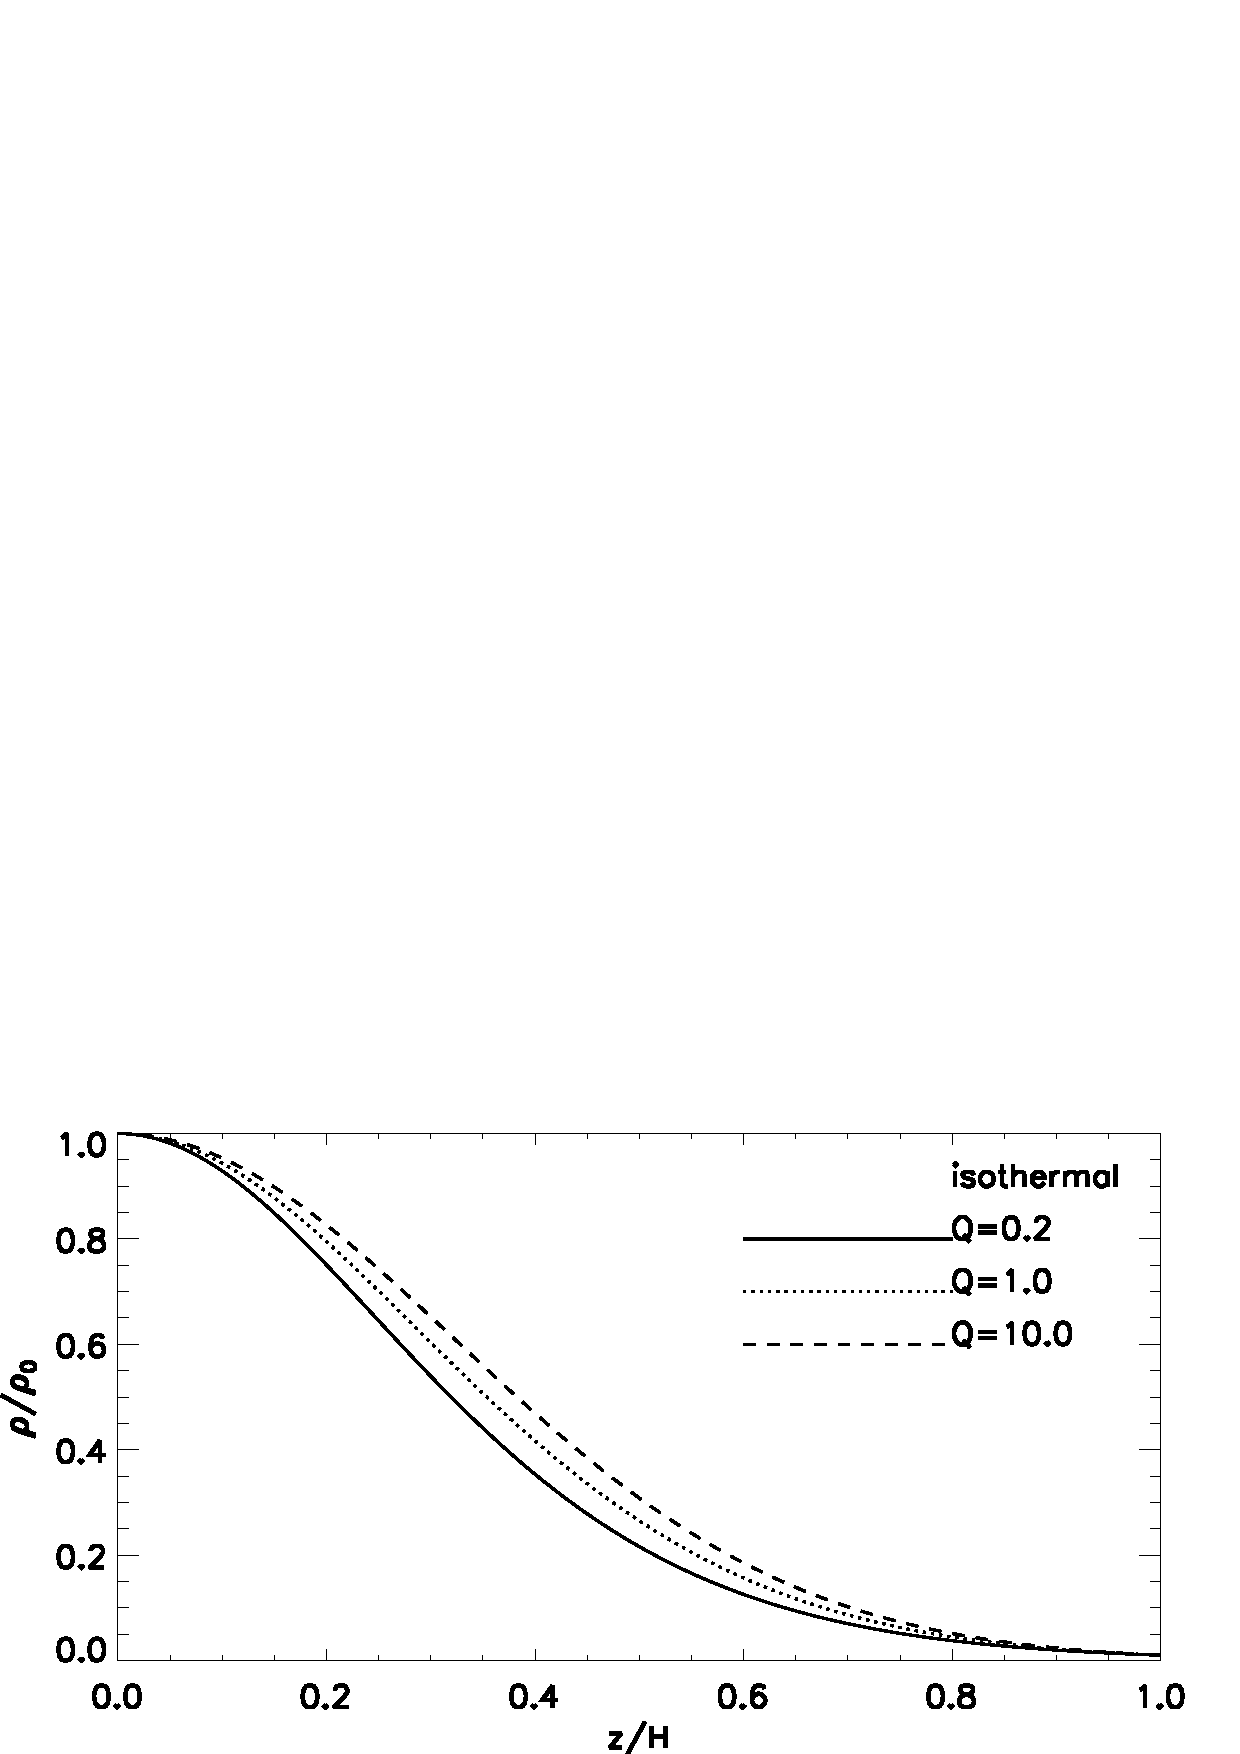
\includegraphics[width=\linewidth]{figures/compare_iso_density}
  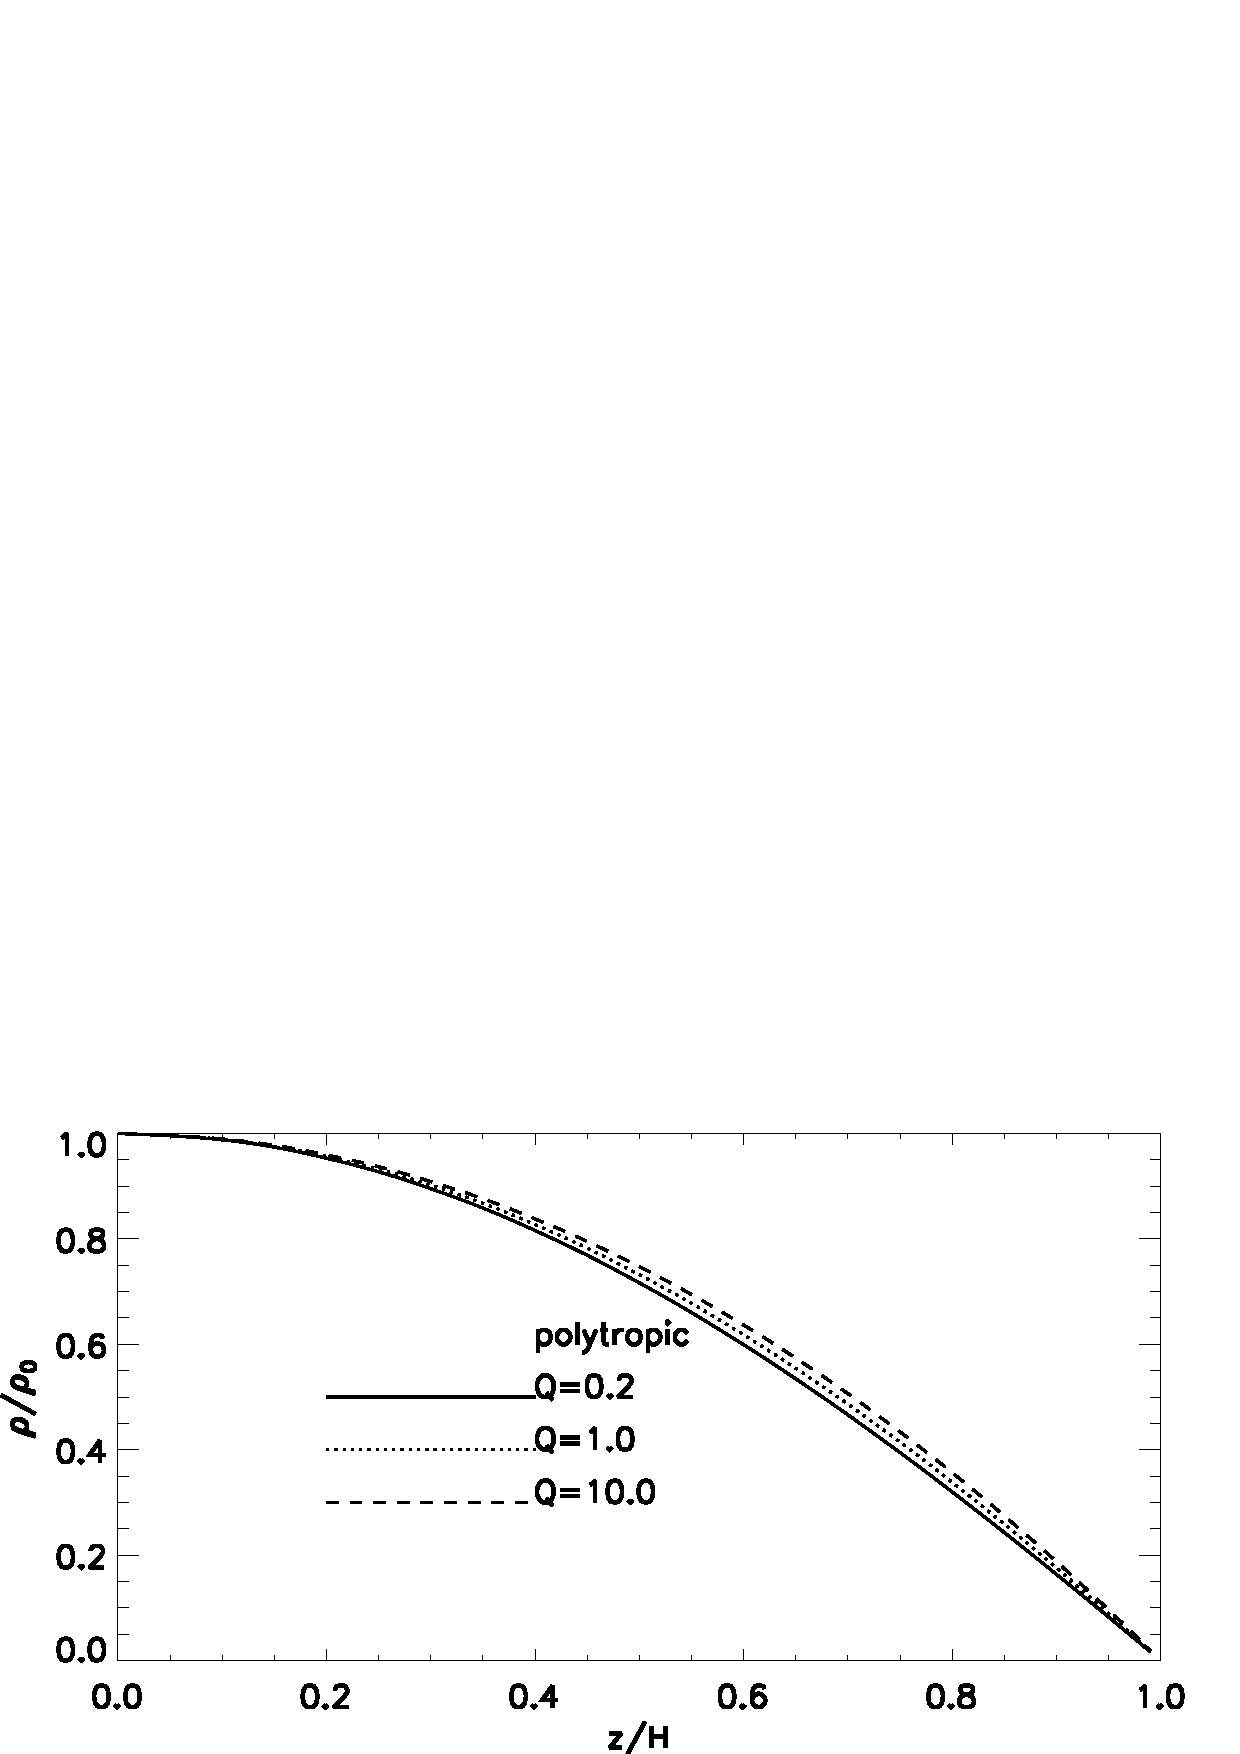
\includegraphics[width=\linewidth]{figures/compare_poly_density}
  \caption{Equilibrium density field from solving Eq. \ref{eqm_eqns1}
    --- \ref{eqm_eqns2} subject to an isothermal (top) and polytropic
    (bottom) equation of state. Note that the vertical co-ordinate is
    normalized differently for convenience. In the isothermal disk,
    $H$ is the characteristic scale-height in the
    non-self-gravitating limit; in the polytropic disk $H$ is the
    disk thickness. \label{eqm_den}}
\end{figure}

\subsection{Resistivity profile}
Following \cite{fleming03}, we adopt the resistivity profile
\begin{align}
  \eta(z) =
  \sqrt{2}\eta_0\left[\exp{\left(-g_+\right)}+\exp{\left(-g_-\right)}\right]^{-1/2},  
\end{align}
where
\begin{align}
  &g_\pm(z) =  \frac{\Sigma_\pm(z)-\Sigma_0}{\Sigma_*}, \\
  &\Sigma_\pm(z) = \int_{\pm z}^\infty\rho(z^\prime)dz^\prime, \label{sigma_pm}
\end{align}
and $\Sigma_0\equiv\Sigma_{\pm}(0)$, so that $g_\pm(0)=0$ and $\eta_0 
= \eta(0)$. The constant $\Sigma_*$ is chosen such that 
\begin{align}
  \cosh{\left(\frac{\Sigma_0}{\Sigma_*}\right)} =
  \left[\frac{\eta_0}{\eta(\infty)}\right]^2,
\end{align}
and we define $\eta_0/\eta(\infty)\equiv A$ as the conductivity
boost factor from the midplane to the disk surface. We remark that
once the equilibrium $\rho$ and $d\rho/dz$ are obtained from
Eq. \ref{eqm_eqns1} --- \ref{eqm_eqns2}, the integration for
Eq. \ref{sigma_pm} can be done implicitly by using the Poisson
equation. 

\subsection{System parameters}
The strength of self-gravity is parametrized by
\begin{align}
  Q \equiv \frac{\Omega^2}{4\pi G\rho_0}
\end{align}
\citep{mamat10}. The plasma $\beta$ measures the inverse strength of
the magnetic field,
\begin{align}
  \beta \equiv \frac{\csmid^2}{v_{A0}^2} =
  \frac{\csmid^2\mu_0\rho_0}{B^2},  
\end{align}
where $v_{A0}$ is the midplane Alfven speed. The strength of
resistivity is measured by the midplane Elsasser number 
\begin{align}
  \Lambda \equiv \frac{v_{A0}^2}{\eta_0\Omega} = \frac{f^2 R_m}{\beta}, 
\end{align}
where the second equality defines the magnetic Reynolds number $R_m$
and $f\equiv \csmid/H\Omega$ is a numerical factor of order unity.  



